% Sequential Fine-Tuning Order Fingerprints -- project presentation
% Compile with pdfLaTeX (Overleaf default). No special fonts required.
\documentclass[aspectratio=169,11pt]{beamer}

\usepackage[T1]{fontenc}
\usepackage{lmodern}
\usepackage{microtype}
\usepackage{amsmath}
\usepackage{booktabs}
\usepackage{colortbl}
\arrayrulecolor{navy}
\heavyrulewidth=0.9pt
\lightrulewidth=0.5pt
\usepackage{graphicx}
\usepackage{adjustbox}
\usepackage{tikz}
\usetikzlibrary{arrows.meta,positioning,calc,fit}

% ---------- Colours ----------
% Goethe-style blue. Change \definecolor{navy} to adjust the whole deck.
\definecolor{navy}{HTML}{00618F}
\definecolor{lightblue}{HTML}{CFE2EE}
\definecolor{midblue}{HTML}{4C93B8}
\definecolor{accent}{HTML}{D9731A}
\definecolor{softgray}{HTML}{EEF4F8}
\definecolor{midgray}{HTML}{5F6B76}
\definecolor{good}{HTML}{2E7D32}
\definecolor{bad}{HTML}{B23A3A}

% ---------- Theme ----------
\usetheme{default}
\renewcommand{\familydefault}{\sfdefault}
\setbeamertemplate{navigation symbols}{}
\setbeamercolor{normal text}{fg=black!85}
\setbeamercolor{structure}{fg=navy}
\setbeamerfont{frametitle}{series=\bfseries,size=\Large}
\setbeamertemplate{frametitle}{%
  \vbox to 0pt{\begin{tikzpicture}[remember picture,overlay]
    \fill[navy] (current page.north west) rectangle ([yshift=-1.55cm]current page.north east);
    \fill[midblue] ([yshift=-1.55cm]current page.north west) rectangle ([yshift=-1.62cm]current page.north east);
  \end{tikzpicture}\vss}%
  \nointerlineskip\vskip3mm
  {\color{white}\usebeamerfont{frametitle}\insertframetitle}\par
  \vskip6.5mm}
\setbeamertemplate{footline}{%
  \vbox{\hbox to \paperwidth{\hspace{1.2em}{\color{lightblue}\rule{\dimexpr\paperwidth-2.4em\relax}{0.6pt}}}\vskip1mm
  \hbox to \paperwidth{\hspace{1.2em}\color{midgray}\footnotesize
  Sequential Fine-Tuning Order Fingerprints\hfill\color{navy}\bfseries\insertframenumber\hspace{1.2em}}\vskip3mm}}
\setbeamertemplate{itemize item}{\color{navy}\raisebox{0.2ex}{\scriptsize$\bullet$}}
\setbeamertemplate{itemize subitem}{\color{midblue}\raisebox{0.1ex}{\tiny$\circ$}}

% ---------- Helper macros ----------
% Folder holding the figure PNGs (relative to this .tex file). Change if needed.
\newcommand{\figdir}{figures/}
% Insert a figure if it exists, otherwise a grey placeholder so the deck still compiles.
\newcommand{\showfig}[2]{%
  \IfFileExists{\figdir#1}%
    {\includegraphics[width=\linewidth,height=#2,keepaspectratio]{\figdir#1}}%
    {\fcolorbox{midgray}{softgray}{\parbox[c][#2][c]{0.9\linewidth}{\centering\color{midgray}
      Figure not found:\\\texttt{\detokenize{#1}}}}}}
% Same, but cuts the given fraction (0-1) off the top of the image (removes the long figure title).
\newcommand{\showfigcrop}[3]{%
  \IfFileExists{\figdir#1}%
    {\adjustbox{trim={0 0 0 {#3\height}}, clip, max height=#2, max width=\linewidth}{\includegraphics{\figdir#1}}}%
    {\fcolorbox{midgray}{softgray}{\parbox[c][#2][c]{0.9\linewidth}{\centering\color{midgray}
      Figure not found:\\\texttt{\detokenize{#1}}}}}}
\newcommand{\hl}[1]{{\color{accent}\bfseries #1}}

\tikzset{
  box/.style={draw=navy, fill=softgray, rounded corners=2pt, align=center, inner sep=5pt, font=\small},
  refbox/.style={box, minimum width=2.4cm},
  arr/.style={-{Stealth[length=2.2mm]}, thick, navy},
}

% ---------- Title info ----------
\title{Sequential Fine-Tuning Order Fingerprints}
\author{Ahmad Ata Ul Haye, Daniel Flick}
\institute{PAMI Practice SS 2026, Goethe Universität Frankfurt}
\date{30.09.2026}

\begin{document}

% ======================================================
{
\setbeamercolor{background canvas}{bg=navy}
\begin{frame}[plain]
  \vbox to 0pt{\begin{tikzpicture}[remember picture,overlay]
    \fill[midblue] (current page.south west) rectangle ([yshift=0.55cm]current page.south east);
    \fill[white] ([xshift=1.2cm,yshift=0.55cm]current page.south west) rectangle ([xshift=3.4cm,yshift=0.65cm]current page.south west);
  \end{tikzpicture}\vss}
  \vspace{1.2cm}
  {\color{white}\bfseries\fontsize{27}{31}\selectfont Sequential Fine-Tuning\\Order Fingerprints\par}
  \vskip4mm{\color{lightblue}\hrule height 1.2pt width 6cm}\vskip4mm
  {\Large\color{lightblue} Can the final model reveal which task it learned last?\par}
  \vfill
  {\color{white}\normalsize \insertauthor\par}
  {\small\color{lightblue} \insertinstitute\par \insertdate\par}
  \vspace{0.9cm}
\end{frame}
}

% ======================================================
\begin{frame}{Research question}
  \begin{columns}[T]
    \begin{column}{0.55\textwidth}
      A network is trained on tasks one after another. Each new task changes the weights.


    \bigskip
    \textbf{Can we predict the final learned task?}

    \bigskip
    \textbf{Can we predict the full training order?}
      
    \bigskip
    \textbf{Explore catastrophic forgetting}

    \bigskip

    \end{column}
    \begin{column}{0.42\textwidth}
      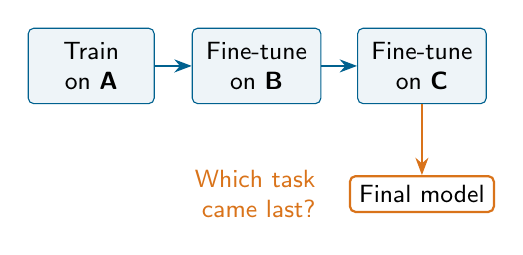
\begin{tikzpicture}
        \node[box, minimum width=1.6cm] (a) at (0,0) {Train\\on \textbf{A}};
        \node[box, minimum width=1.6cm] (b) at (2.1,0) {Fine-tune\\on \textbf{B}};
        \node[box, minimum width=1.6cm] (c) at (4.2,0) {Fine-tune\\on \textbf{C}};
        \draw[arr] (a)--(b); \draw[arr] (b)--(c);
        \node[draw=accent, thick, rounded corners=2pt, align=center, font=\small, below=9mm of c] (f) {Final model};
        \draw[arr, accent] (c)--(f);
        \node[font=\small, color=accent, left=3mm of f, align=right] {Which task\\came last?};
      \end{tikzpicture}
    \end{column}
  \end{columns}
\end{frame}

% ======================================================
\begin{frame}{Setup: three small classification tasks}
  Each task is a 5-class problem built from CIFAR-100 classes. All tasks share one ResNet18 backbone; every task has its own 5-class head.

  \bigskip
  \centering
  \begin{tabular}{@{}llp{7.5cm}@{}}
    \toprule
    \textbf{Task} & \textbf{Theme} & \textbf{Classes}\\
    \midrule
    \hl{A} & Aquatic animals & beaver, dolphin, otter, seal, whale\\[2pt]
    \hl{B} & Electronic / office devices & clock, keyboard, lamp, telephone, television\\[2pt]
    \hl{C} & Vehicles & bicycle, bus, motorcycle, pickup truck, train\\
    \bottomrule
  \end{tabular}

  \bigskip
  \raggedright
  Six task orders are tested: all permutations of A, B, C. \\
  The \hl{actual last task} of an order is simply its final element.
\end{frame}

% ======================================================
\begin{frame}{How the sequential models are trained}
  \begin{columns}[T]
    \begin{column}{0.48\textwidth}
      For an order such as $A \to B \to C$:
      \begin{enumerate}
        \item Train backbone and A-head on A.
        \item Freeze the A-head, add a B-head, train on B.
        \item Freeze A- and B-heads, add a C-head, train on C.
      \end{enumerate}
      \medskip
       A checkpoint is saved after every stage; the last one is the \hl{final sequential model}.
    \end{column}
    \begin{column}{0.5\textwidth}
      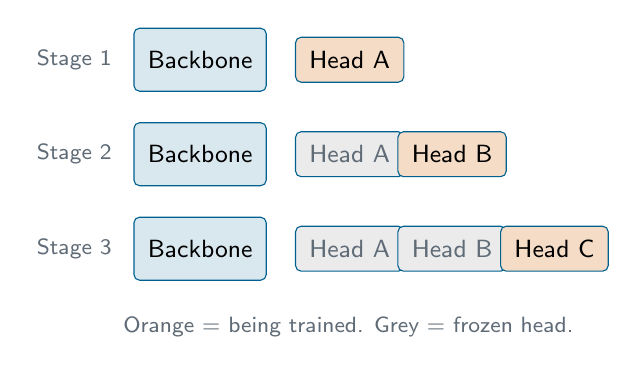
\begin{tikzpicture}[x=1cm,y=1cm]
        \foreach \s/\y in {1/2.4, 2/1.2, 3/0} {
          \node[font=\footnotesize, color=midgray, anchor=east] at (0.1,\y) {Stage \s};
          \node[box, minimum width=1.6cm, minimum height=0.8cm, fill=navy!15] at (1.1,\y) (bb\s) {Backbone};
        }
        \node[box, fill=accent!25] at (3.0,2.4) {Head A};
        \node[box, fill=black!8, text=midgray] at (3.0,1.2) {Head A};
        \node[box, fill=accent!25] at (4.3,1.2) {Head B};
        \node[box, fill=black!8, text=midgray] at (3.0,0) {Head A};
        \node[box, fill=black!8, text=midgray] at (4.3,0) {Head B};
        \node[box, fill=accent!25] at (5.6,0) {Head C};
        \node[font=\footnotesize, color=midgray, anchor=north west] at (0.0,-0.75) {Orange = being trained. Grey = frozen head.};
      \end{tikzpicture}
    \end{column}
  \end{columns}
\end{frame}

% ======================================================
\begin{frame}{The fingerprint test}
  \begin{columns}[T]
    \begin{column}{0.5\textwidth}
      \textbf{Reference models:} three models, each trained only on A, B or C (Single-A, Single-B, Single-C).

      \medskip
      \textbf{Test:} compare the final sequential model with each reference, and pick the reference that looks most similar. That task is the \hl{predicted last task}.

      \medskip
      A prediction is correct if it equals the last element of the order.

      \medskip
      Random guessing gives $1/3 = 33.3\%$.
    \end{column}
    \begin{column}{0.48\textwidth}
      \centering
      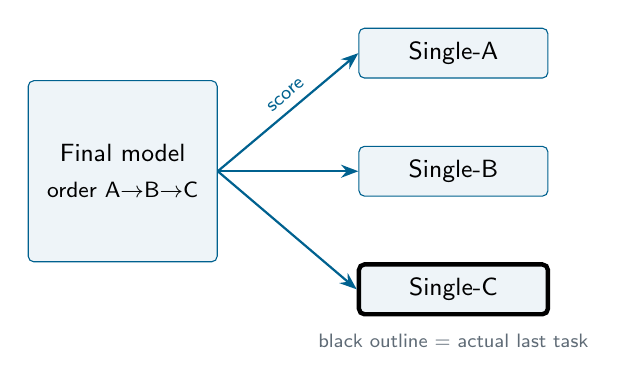
\begin{tikzpicture}
        \node[box, minimum height=2.3cm, minimum width=2.4cm] (m) at (0,0) {Final model\\[2pt]{\footnotesize order A$\to$B$\to$C}};
        \node[refbox] (ra) at (4.2,1.5) {Single-A};
        \node[refbox] (rb) at (4.2,0) {Single-B};
        \node[refbox, line width=1.6pt, draw=black] (rc) at (4.2,-1.5) {Single-C};
        \draw[arr] (m.east) -- node[above, font=\scriptsize, sloped, pos=0.55] {score} (ra.west);
        \draw[arr] (m.east) -- (rb.west);
        \draw[arr] (m.east) -- (rc.west);
        \node[font=\scriptsize, color=midgray, below=1mm of rc, align=center] {black outline = actual last task};
      \end{tikzpicture}
    \end{column}
  \end{columns}
\end{frame}

% ======================================================
\begin{frame}{Methods overview: predictors and diagnostics}
  \footnotesize
  \centering
  \renewcommand{\arraystretch}{1.2}
  \begin{tabular}{@{}p{3.1cm}p{6.4cm}p{4.1cm}@{}}
    \toprule
    \textbf{Method} & \textbf{What is compared} & \textbf{Prediction rule}\\
    \midrule
    \multicolumn{3}{@{}l}{\textcolor{navy}{\textbf{Fingerprint predictors}}}\\
    Weight distance (L2) & Final model vs.\ each reference & Smallest distance\\
    CKA & Feature structure on a fixed image set & Highest similarity\\
    Feature drift & Feature vectors, image by image & Smallest drift\\
    Weight matching & Weights after undoing neuron reordering & Smallest L2, highest cosine\\
    Fisher trace & Curvature of the final model alone & Both directions tested\\
    \midrule
    \multicolumn{3}{@{}l}{\textcolor{navy}{\textbf{Forgetting diagnostics}}}\\
    Forgetting & Accuracy after learning vs.\ final accuracy & -\\
    \bottomrule
  \end{tabular}
\end{frame}


% ======================================================
\begin{frame}{Result: how often is the last task predicted correctly?}
  \begin{columns}[T]
    \begin{column}{0.64\textwidth}
      \centering
      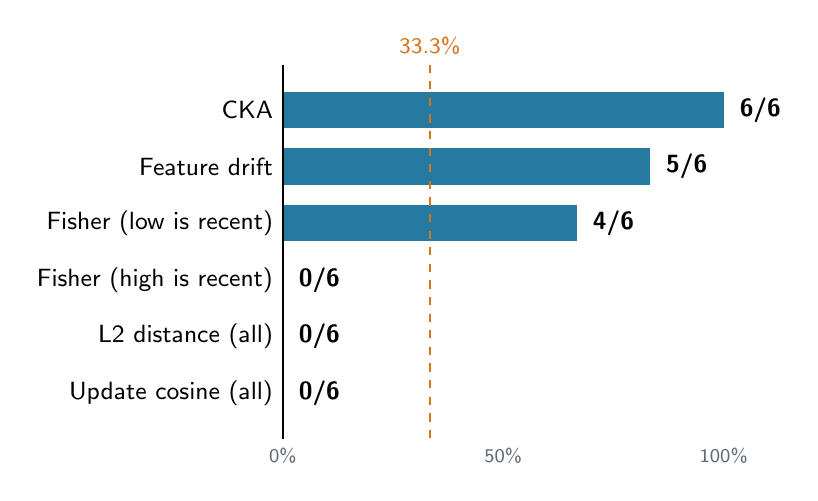
\begin{tikzpicture}[x=1cm,y=0.72cm]
        \def\W{5.6}
        \foreach \lab/\val/\cnt/\col [count=\i] in {%
          {CKA/100/6/navy},
          {Feature drift/83.3/5/navy},
          {Fisher (low is recent)/66.7/4/navy},
          {Fisher (high is recent)/0/0/bad},
          {L2 distance (all)/0/0/bad},
          {Update cosine (all)/0/0/bad}} {
          \pgfmathsetmacro{\y}{-\i}
          \node[anchor=east, font=\small] at (0,\y) {\lab};
          \pgfmathsetmacro{\w}{\W*\val/100}
          \ifdim\w pt>0pt
            \fill[\col!85] (0,\y-0.32) rectangle (\w,\y+0.32);
          \fi
          \node[anchor=west, font=\small\bfseries] at (\w+0.08,\y) {\cnt/6};
        }
        \draw[thick] (0,-0.2) -- (0,-6.8);
        \draw[dashed, accent, thick] (\W/3,-0.2) -- (\W/3,-6.8);
        \node[accent, font=\footnotesize, anchor=south] at (\W/3,-0.2) {33.3\%};
        \foreach \p in {0,50,100} { \node[font=\scriptsize, color=midgray] at (\W*\p/100,-7.1) {\p\%}; }
      \end{tikzpicture}
    \end{column}
    \begin{column}{0.34\textwidth}
      \small
      \begin{itemize}
        \item CKA is right in every order.
        \item Feature drift misses one.
        \item Fisher works only as ``lowest = most recent'' (total and backbone).
        \item L2 and cosine are wrong in every order, also after matching.
      \end{itemize}
      \vspace{1mm}
      {\scriptsize\color{midgray} Dashed: 33.3\% baseline. 20 epochs/task, \texttt{all\_test}, seed 42.}
    \end{column}
  \end{columns}
\end{frame}

% ======================================================
\begin{frame}{Prediction matrix: every order, every method}
  \centering
  \showfig{prediction_matrix.png}{4.1cm}

  \vspace{1mm}
  \raggedright\small
  Rows are orders, columns are methods, cells show the predicted task. \textcolor{good}{Green} is correct, \textcolor{bad}{red} is wrong.

  \smallskip
  In every L2 and cosine column the predicted task is the \hl{first} task of the order, never the last.
\end{frame}

% ======================================================
\begin{frame}{CKA separates the last task clearly}
  \begin{columns}[T]
    \begin{column}{0.66\textwidth}
      Asks: is the structure of the representation similar?
      Highest CKA predicts the last task.
      \bigskip

      \showfigcrop{cka_similarity.png}{5.3cm}{0.13}
    \end{column}
    \begin{column}{0.31\textwidth}
      \footnotesize

      Bars show CKA between the final model and Single-A, B, C. Outline marks the actual last task.
      \begin{itemize}
        \item The outlined bar is the highest in all six orders.
        \item Last-task CKA lies between 0.63 and 0.75.
        \item The other two references lie between 0.19 and 0.43.
      \end{itemize}
      The gap is large, not a near tie.
    \end{column}
  \end{columns}
\end{frame}

% ======================================================
\begin{frame}{Feature drift}
  \begin{columns}[T]
    \begin{column}{0.66\textwidth}
      Asks: did the individual feature vectors move?
      Lowest drift predicts the last task.
      \bigskip

      \showfigcrop{feature_drift.png}{5.3cm}{0.13}
    \end{column}
    \begin{column}{0.31\textwidth}
      \footnotesize
      Lower drift means more similar features. Outline marks the actual last task.
      \begin{itemize}
        \item The outlined bar is the lowest in 5 of 6 orders.
        \item The miss is B$\to$C$\to$A: Single-B (0.571) is just below Single-A (0.579).
        \item All values lie between 0.54 and 0.62, so margins are small compared with CKA.
      \end{itemize}
    \end{column}
  \end{columns}
\end{frame}

% ======================================================
\begin{frame}{Weight distance points at the first task}
  \begin{columns}[T]
    \begin{column}{0.62\textwidth}
      \showfigcrop{weight_distance_scores.png}{5.3cm}{0.06}
    \end{column}
    \begin{column}{0.35\textwidth}
      \footnotesize
      L2 distance from each final model to the three references, for the full model (top) and the backbone (bottom). Outline marks the actual last task.
      \begin{itemize}
        \item In every order the \hl{closest} reference is the \hl{first} task.
        \item The last task is never the closest: 0 of 6.
        \item Full model and backbone give the same picture.
      \end{itemize}
    \end{column}
  \end{columns}
\end{frame}

% ======================================================
\begin{frame}{Weight matching changes nothing}
  \begin{columns}[T]
    \begin{column}{0.64\textwidth}
      \showfigcrop{weight_matching_before_after.png}{4.8cm}{0.07}
    \end{column}
    \begin{column}{0.34\textwidth}
      \small
      Each row is one final model and one reference. Dots: before matching. Crosses: after.
      \begin{itemize}
        \item Dots and crosses coincide everywhere: distances did not change.
        \item This fits the expected identity permutation with a shared initialization.
        \item The cosine of weight updates is highest for the first task, so it fails like L2.
      \end{itemize}
    \end{column}
  \end{columns}
\end{frame}


% ======================================================
\begin{frame}{Fisher information}
  \begin{columns}[T]
    \begin{column}{0.52\textwidth}
      \showfig{fisher_hypothesis_accuracy.png}{4.8cm}
    \end{column}
    \begin{column}{0.45\textwidth}
      \small
      \begin{itemize}
        \item \texttt{low\_is\_recent}: 4/6 for both total and backbone Fisher.
        \item \texttt{high\_is\_recent}: 0/6.
        \item The two misses are the orders that start with A. There, the first task A has the lowest trace and is predicted.
        \item So this method predicts A in 4 of 6 orders, and A is last in only 2.
        \item Full training order: 1/6 correct, chance is 1/6.
      \end{itemize}
    \end{column}
  \end{columns}
\end{frame}

% ======================================================

\begin{frame}{Forgetting}
  \begin{columns}[T]
    \begin{column}{0.66\textwidth}
      \showfigcrop{forgetting_by_order.png}{5.3cm}{0.07}
    \end{column}
    \begin{column}{0.31\textwidth}
      \footnotesize
      $\text{forgetting}(T)=\text{acc. after learning }T-\text{final acc. on }T$
      \begin{itemize}
        \item Earlier tasks lose about 0.23 to 0.45 accuracy.
        \item The last task shows zero forgetting in every order.
        \item That is by construction: for the last task, ``after learning'' and ``final'' are the same checkpoint.
      \end{itemize}
      So forgetting gives no independent evidence of a fingerprint.
    \end{column}
  \end{columns}
\end{frame}


% ======================================================
\begin{frame}{Hypotheses and outcome}
  \small
  \renewcommand{\arraystretch}{1.3}
  \begin{tabular}{@{}p{0.6cm}p{4.6cm}p{6.6cm}@{}}
    \toprule
    & \textbf{Hypothesis} & \textbf{Outcome so far}\\
    \midrule
    H1 & Can we predict the final learned task? & CKA 6/6, feature drift 5/6, Fisher (low is recent) 4/6. L2 and cosine 0/6.\\
    H2 & Can we predict the full training order? & In combination of CKA and weight distance\\
    H3 & Explore catastrophic forgetting & Accuracies drop sharply for older tasks\\
    \bottomrule
  \end{tabular}
\end{frame}

% ======================================================
\begin{frame}{Limitations}
  \begin{itemize}
    \item \textbf{One training run}. No estimate of run-to-run variation.
     \bigskip 
    \item \textbf{Only 3 Tasks per Order.} 
     \bigskip
     \item \textbf{Fisher predictions are concentrated on A} (4 of 6 orders).
     \bigskip
    \item \textbf{Small tasks.} 5 classes each, from CIFAR-100; the tasks may be too similar or too different.
  \end{itemize}
\end{frame}

% ======================================================
\begin{frame}{Conclusions}
      \textbf{Conclusions}
      \bigskip
      \begin{itemize}
        \item The last task is detectable in the \hl{representations} (CKA, feature drift) and, less reliably, in the \hl{curvature} (Fisher).
        \item Weight distance and update cosine point at the first task.
        \item Forgetting adds no independent evidence.
      \end{itemize}
\end{frame}

% ======================================================
\begin{frame}{Questions}
    \centering
    \textbf{Thank you for your attention!}
    \bigskip
    \textbf{Any Questions?}
\end{frame}

\end{document}